\documentclass{extbook}[14pt]
\usepackage{multicol, enumerate, enumitem, hyperref, color, soul, setspace, parskip, fancyhdr, amssymb, amsthm, amsmath, bbm, latexsym, units, mathtools}
\everymath{\displaystyle}
\usepackage[headsep=0.5cm,headheight=0cm, left=1 in,right= 1 in,top= 1 in,bottom= 1 in]{geometry}
\usepackage{dashrule}  % Package to use the command below to create lines between items
\newcommand{\litem}[1]{\item #1

\rule{\textwidth}{0.4pt}}
\pagestyle{fancy}
\lhead{}
\chead{Answer Key for Progress Quiz 4 Version C}
\rhead{}
\lfoot{6286-1986}
\cfoot{}
\rfoot{Fall 2020}
\begin{document}
\textbf{This key should allow you to understand why you choose the option you did (beyond just getting a question right or wrong). \href{https://xronos.clas.ufl.edu/mac1105spring2020/courseDescriptionAndMisc/Exams/LearningFromResults}{More instructions on how to use this key can be found here}.}

\textbf{If you have a suggestion to make the keys better, \href{https://forms.gle/CZkbZmPbC9XALEE88}{please fill out the short survey here}.}

\textit{Note: This key is auto-generated and may contain issues and/or errors. The keys are reviewed after each exam to ensure grading is done accurately. If there are issues (like duplicate options), they are noted in the offline gradebook. The keys are a work-in-progress to give students as many resources to improve as possible.}

\rule{\textwidth}{0.4pt}

\begin{enumerate}\litem{
Choose the graph of the equation below.
\[ f(x) = \frac{-1}{(x + 3)^2} - 1 \]
The solution is the graph below, which is option C.
\begin{center}
    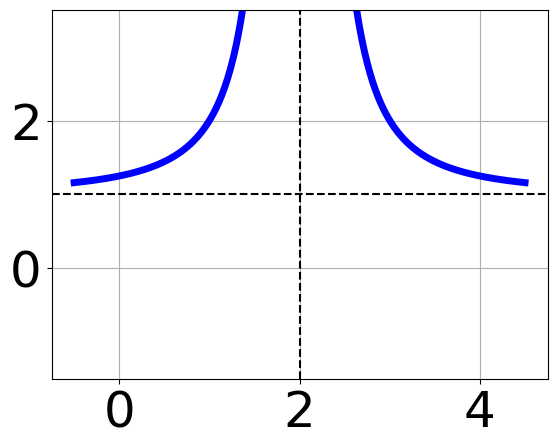
\includegraphics[width=0.3\textwidth]{../Figures/rationalEquationToGraphCC.png}
\end{center}\begin{enumerate}[label=\Alph*.]
\begin{multicols}{2}
\item 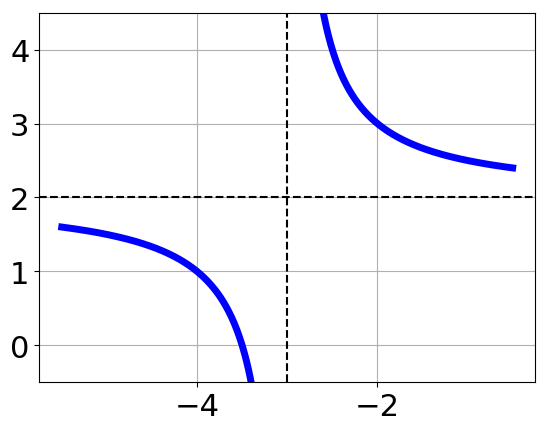
\includegraphics[width = 0.3\textwidth]{../Figures/rationalEquationToGraphAC.png}
\item 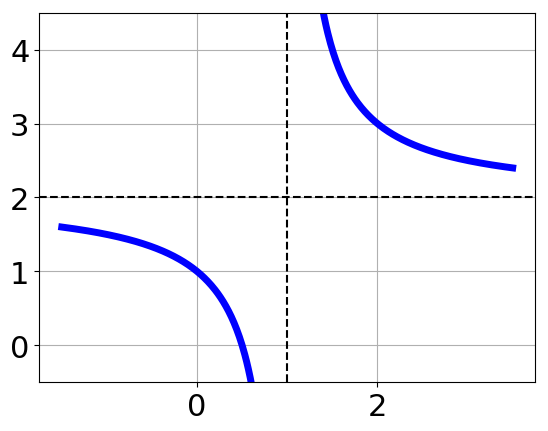
\includegraphics[width = 0.3\textwidth]{../Figures/rationalEquationToGraphBC.png}
\item 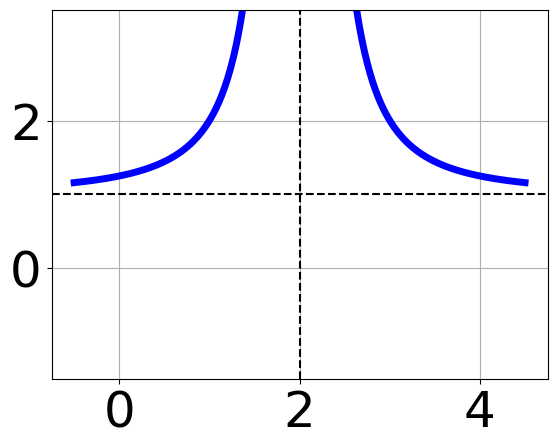
\includegraphics[width = 0.3\textwidth]{../Figures/rationalEquationToGraphCC.png}
\item 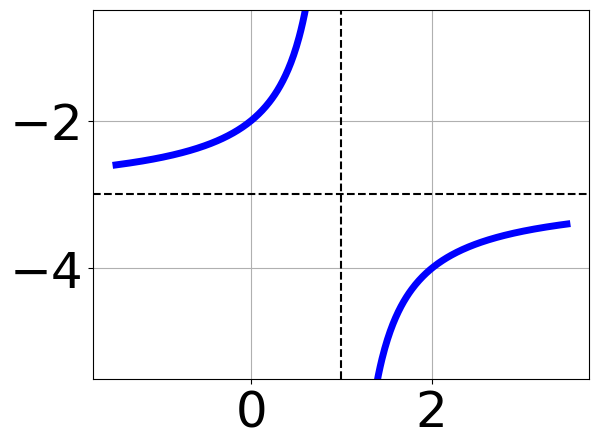
\includegraphics[width = 0.3\textwidth]{../Figures/rationalEquationToGraphDC.png}
\end{multicols}\item None of the above.\end{enumerate}
\textbf{General Comment:} Remember that the general form of a basic rational equation is $ f(x) = \frac{a}{(x-h)^n} + k$, where $a$ is the leading coefficient (and in this case, we assume is either $1$ or $-1$), $n$ is the degree (in this case, either $1$ or $2$), and $(h, k)$ is the intersection of the asymptotes.
}
\litem{
Choose the equation of the function graphed below.

\begin{center}
    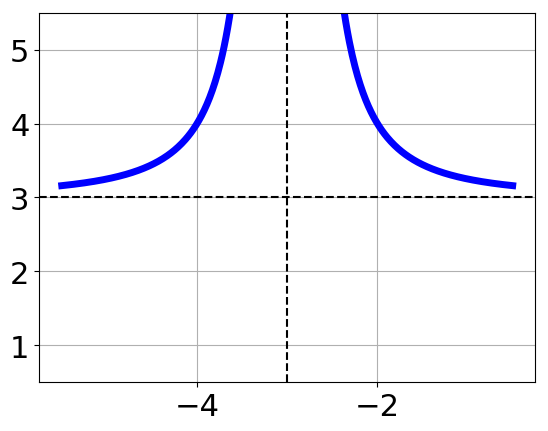
\includegraphics[width=0.5\textwidth]{../Figures/rationalGraphToEquationC.png}
\end{center}



The solution is \( f(x) = \frac{-1}{x - 3} - 2 \), which is option B.\begin{enumerate}[label=\Alph*.]
\item \( f(x) = \frac{1}{x + 3} - 2 \)

Corresponds to using the general form $f(x) = \frac{a}{x+h}+k$ and the opposite leading coefficient.
\item \( f(x) = \frac{-1}{x - 3} - 2 \)

This is the correct option.
\item \( f(x) = \frac{-1}{(x - 3)^2} - 2 \)

Corresponds to thinking the graph was a shifted version of $\frac{1}{x^2}$.
\item \( f(x) = \frac{1}{(x + 3)^2} - 2 \)

Corresponds to thinking the graph was a shifted version of $\frac{1}{x^2}$, using the general form $f(x) = \frac{a}{x+h}+k$, and the opposite leading coefficient.
\item \( \text{None of the above} \)

This corresponds to believing the vertex of the graph was not correct.
\end{enumerate}

\textbf{General Comment:} Remember that the general form of a basic rational equation is $ f(x) = \frac{a}{(x-h)^n} + k$, where $a$ is the leading coefficient (and in this case, we assume is either $1$ or $-1$), $n$ is the degree (in this case, either $1$ or $2$), and $(h, k)$ is the intersection of the asymptotes.
}
\litem{
Solve the rational equation below. Then, choose the interval(s) that the solution(s) belongs to.
\[ \frac{7}{4x -4} + 2 = \frac{-5}{-16x + 16} \]
The solution is \( x = 0.281 \), which is option B.\begin{enumerate}[label=\Alph*.]
\item \( \text{All solutions lead to invalid or complex values in the equation.} \)

This corresponds to thinking $x = 0.281$ leads to dividing by zero in the original equation, which it does not.
\item \( x \in [0.28,1.28] \)

* $x = 0.281$, which is the correct option.
\item \( x_1 \in [-2.8, -1.1] \text{ and } x_2 \in [-0.72,2.28] \)

$x = -1.719 \text{ and } x = 0.281$, which corresponds to getting the correct solution and believing there should be a second solution to the equation.
\item \( x_1 \in [-0.8, -0.3] \text{ and } x_2 \in [-0.72,2.28] \)

$x = -0.500 \text{ and } x = 0.281$, which corresponds to getting the correct solution and believing there should be a second solution to the equation.
\item \( x \in [-2.8,-1.1] \)

$x = -1.719$, which corresponds to not distributing the factor $4x -4$ correctly when trying to eliminate the fraction.
\end{enumerate}

\textbf{General Comment:} Distractors are different based on the number of solutions. Remember that after solving, we need to make sure our solution does not make the original equation divide by zero!
}
\litem{
Determine the domain of the function below.
\[ f(x) = \frac{3}{25x^{2} +40 x + 15} \]
The solution is \( \text{All Real numbers except } x = -1.000 \text{ and } x = -0.600. \), which is option A.\begin{enumerate}[label=\Alph*.]
\item \( \text{All Real numbers except } x = a \text{ and } x = b, \text{ where } a \in [-1.87, -0.79] \text{ and } b \in [-0.87, -0.22] \)

All Real numbers except $x = -1.000$ and $x = -0.600$, which is the correct option.
\item \( \text{All Real numbers.} \)

This corresponds to thinking the denominator has complex roots or that rational functions have a domain of all Real numbers.
\item \( \text{All Real numbers except } x = a, \text{ where } a \in [-25.39, -24.25] \)

All Real numbers except $x = -25.000$, which corresponds to removing a distractor value from the denominator.
\item \( \text{All Real numbers except } x = a \text{ and } x = b, \text{ where } a \in [-25.39, -24.25] \text{ and } b \in [-15.38, -14.04] \)

All Real numbers except $x = -25.000$ and $x = -15.000$, which corresponds to not factoring the denominator correctly.
\item \( \text{All Real numbers except } x = a, \text{ where } a \in [-1.87, -0.79] \)

All Real numbers except $x = -1.000$, which corresponds to removing only 1 value from the denominator.
\end{enumerate}

\textbf{General Comment:} Recall that dividing by zero is not a real number. Therefore the domain is all real numbers \textbf{except} those that make the denominator 0.
}
\litem{
Solve the rational equation below. Then, choose the interval(s) that the solution(s) belongs to.
\[ \frac{2x}{-5x + 2} + \frac{-2x^{2}}{-35x^{2} +44 x -12} = \frac{-3}{7x -6} \]
The solution is \( \text{There are two solutions: } x = 0.250 \text{ and } x = 2.000 \), which is option D.\begin{enumerate}[label=\Alph*.]
\item \( x_1 \in [0.25, 0.38] \text{ and } x_2 \in [-1.6,1.4] \)


\item \( \text{All solutions lead to invalid or complex values in the equation.} \)


\item \( x \in [0.57,0.86] \)


\item \( x_1 \in [0.25, 0.38] \text{ and } x_2 \in [2,6] \)

* $x = 0.250 \text{ and } x = 2.000$, which is the correct option.
\item \( x \in [1.49,2.35] \)


\end{enumerate}

\textbf{General Comment:} Distractors are different based on the number of solutions. Remember that after solving, we need to make sure our solution does not make the original equation divide by zero!
}
\litem{
Choose the equation of the function graphed below.

\begin{center}
    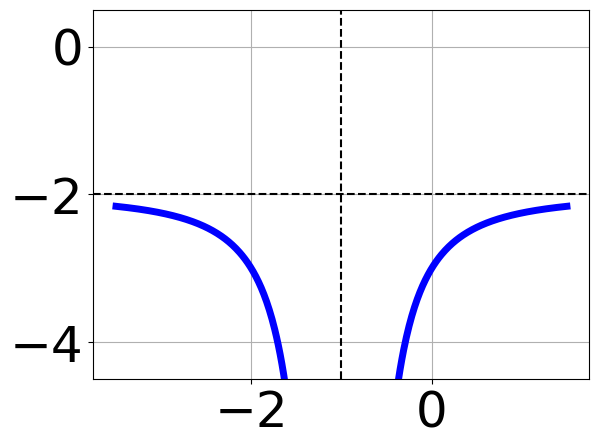
\includegraphics[width=0.5\textwidth]{../Figures/rationalGraphToEquationCopyC.png}
\end{center}



The solution is \( f(x) = \frac{-1}{(x + 2)^2} + 1 \), which is option A.\begin{enumerate}[label=\Alph*.]
\item \( f(x) = \frac{-1}{(x + 2)^2} + 1 \)

This is the correct option.
\item \( f(x) = \frac{1}{x - 2} + 1 \)

Corresponds to thinking the graph was a shifted version of $\frac{1}{x}$, using the general form $f(x) = \frac{a}{(x+h)^2}+k$, and the opposite leading coefficient.
\item \( f(x) = \frac{-1}{x + 2} + 1 \)

Corresponds to thinking the graph was a shifted version of $\frac{1}{x}$.
\item \( f(x) = \frac{1}{(x - 2)^2} + 1 \)

Corresponds to using the general form $f(x) = \frac{a}{(x+h)^2}+k$ and the opposite leading coefficient.
\item \( \text{None of the above} \)

This corresponds to believing the vertex of the graph was not correct.
\end{enumerate}

\textbf{General Comment:} Remember that the general form of a basic rational equation is $ f(x) = \frac{a}{(x-h)^n} + k$, where $a$ is the leading coefficient (and in this case, we assume is either $1$ or $-1$), $n$ is the degree (in this case, either $1$ or $2$), and $(h, k)$ is the intersection of the asymptotes.
}
\litem{
Choose the graph of the equation below.
\[ f(x) = \frac{1}{x + 2} - 3 \]
The solution is the graph below, which is option A.
\begin{center}
    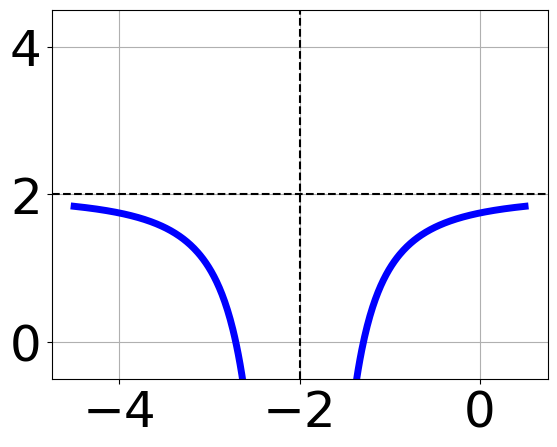
\includegraphics[width=0.3\textwidth]{../Figures/rationalEquationToGraphCopyAC.png}
\end{center}\begin{enumerate}[label=\Alph*.]
\begin{multicols}{2}
\item 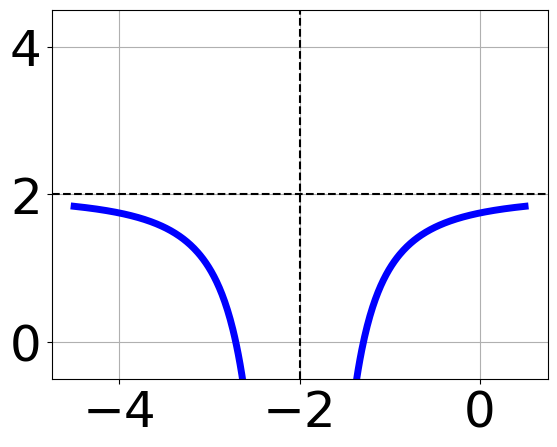
\includegraphics[width = 0.3\textwidth]{../Figures/rationalEquationToGraphCopyAC.png}
\item 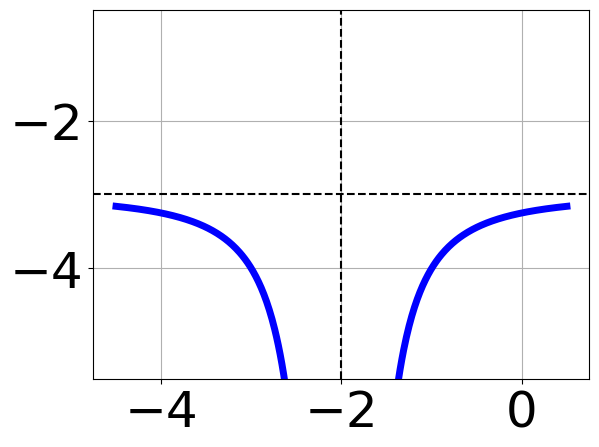
\includegraphics[width = 0.3\textwidth]{../Figures/rationalEquationToGraphCopyBC.png}
\item 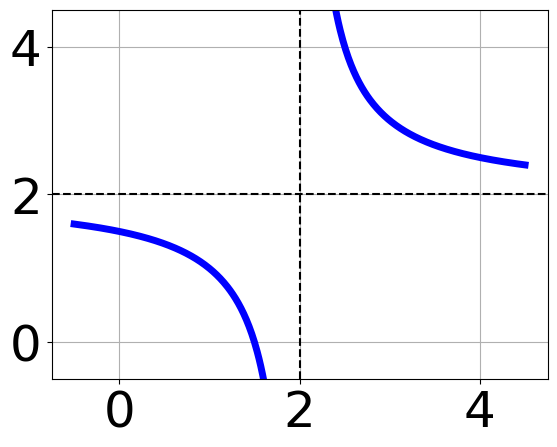
\includegraphics[width = 0.3\textwidth]{../Figures/rationalEquationToGraphCopyCC.png}
\item 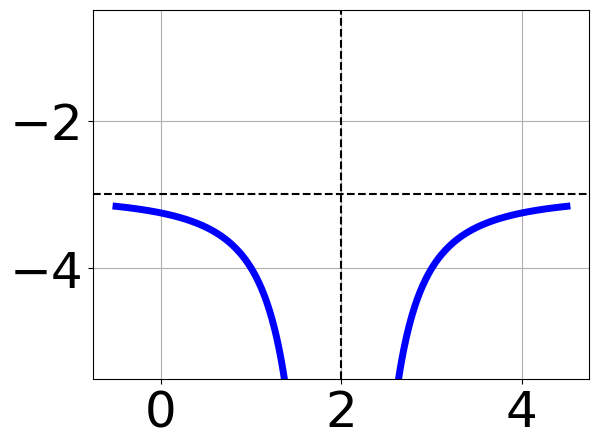
\includegraphics[width = 0.3\textwidth]{../Figures/rationalEquationToGraphCopyDC.png}
\end{multicols}\item None of the above.\end{enumerate}
\textbf{General Comment:} Remember that the general form of a basic rational equation is $ f(x) = \frac{a}{(x-h)^n} + k$, where $a$ is the leading coefficient (and in this case, we assume is either $1$ or $-1$), $n$ is the degree (in this case, either $1$ or $2$), and $(h, k)$ is the intersection of the asymptotes.
}
\litem{
Solve the rational equation below. Then, choose the interval(s) that the solution(s) belongs to.
\[ \frac{9}{-6x + 4} + -9 = \frac{-3}{-54x + 36} \]
The solution is \( x = 0.494 \), which is option C.\begin{enumerate}[label=\Alph*.]
\item \( x_1 \in [0.39, 0.47] \text{ and } x_2 \in [0.49,1.49] \)

$x = 0.444 \text{ and } x = 0.494$, which corresponds to getting the correct solution and believing there should be a second solution to the equation.
\item \( x_1 \in [-0.87, -0.82] \text{ and } x_2 \in [0.49,1.49] \)

$x = -0.840 \text{ and } x = 0.494$, which corresponds to getting the correct solution and believing there should be a second solution to the equation.
\item \( x \in [0.49,1.49] \)

* $x = 0.494$, which is the correct option.
\item \( x \in [-0.87,-0.82] \)

$x = -0.840$, which corresponds to not distributing the factor $-6x + 4$ correctly when trying to eliminate the fraction.
\item \( \text{All solutions lead to invalid or complex values in the equation.} \)

This corresponds to thinking $x = 0.494$ leads to dividing by zero in the original equation, which it does not.
\end{enumerate}

\textbf{General Comment:} Distractors are different based on the number of solutions. Remember that after solving, we need to make sure our solution does not make the original equation divide by zero!
}
\litem{
Solve the rational equation below. Then, choose the interval(s) that the solution(s) belongs to.
\[ \frac{5x}{-2x -3} + \frac{-2x^{2}}{-8x^{2} -2 x + 15} = \frac{-5}{4x -5} \]
The solution is \( \text{There are two solutions: } x = -0.361 \text{ and } x = 2.306 \), which is option E.\begin{enumerate}[label=\Alph*.]
\item \( \text{All solutions lead to invalid or complex values in the equation.} \)


\item \( x \in [0.58,1.76] \)


\item \( x_1 \in [-0.99, -0.09] \text{ and } x_2 \in [-2.5,0.5] \)


\item \( x \in [1.75,2.45] \)


\item \( x_1 \in [-0.99, -0.09] \text{ and } x_2 \in [0.31,6.31] \)

* $x = -0.361 \text{ and } x = 2.306$, which is the correct option.
\end{enumerate}

\textbf{General Comment:} Distractors are different based on the number of solutions. Remember that after solving, we need to make sure our solution does not make the original equation divide by zero!
}
\litem{
Determine the domain of the function below.
\[ f(x) = \frac{6}{30x^{2} -11 x -30} \]
The solution is \( \text{All Real numbers except } x = -0.833 \text{ and } x = 1.200. \), which is option A.\begin{enumerate}[label=\Alph*.]
\item \( \text{All Real numbers except } x = a \text{ and } x = b, \text{ where } a \in [-4.83, 0.17] \text{ and } b \in [-0.8, 2.2] \)

All Real numbers except $x = -0.833$ and $x = 1.200$, which is the correct option.
\item \( \text{All Real numbers except } x = a \text{ and } x = b, \text{ where } a \in [-33, -29] \text{ and } b \in [30, 31] \)

All Real numbers except $x = -30.000$ and $x = 30.000$, which corresponds to not factoring the denominator correctly.
\item \( \text{All Real numbers except } x = a, \text{ where } a \in [-4.83, 0.17] \)

All Real numbers except $x = -0.833$, which corresponds to removing only 1 value from the denominator.
\item \( \text{All Real numbers.} \)

This corresponds to thinking the denominator has complex roots or that rational functions have a domain of all Real numbers.
\item \( \text{All Real numbers except } x = a, \text{ where } a \in [-33, -29] \)

All Real numbers except $x = -30.000$, which corresponds to removing a distractor value from the denominator.
\end{enumerate}

\textbf{General Comment:} Recall that dividing by zero is not a real number. Therefore the domain is all real numbers \textbf{except} those that make the denominator 0.
}
\end{enumerate}

\end{document}